
\documentclass[12pt,letterpaper]{article}
\usepackage[spanish]{babel}  		 % Idioma
\usepackage[utf8]{inputenc}      % Codificación
\usepackage{geometry}				     % Margenes
\usepackage{setspace}            % Interlineado
\usepackage{fancyhdr}
\usepackage{graphicx}
\usepackage{caption}   % Para personalizar leyendas
\usepackage[T1]{fontenc}         % Fuentes
\usepackage{times}               % Fuente Times New Roman
\usepackage{titlesec}            % Formato de secciones
\usepackage{titletoc}			% Formato del indice
\usepackage[backend=biber, style=apa]{biblatex} % Para usar bibliografia
\usepackage{csquotes}
\usepackage{enumitem}			% para las listas 
\usepackage[nopatch=item]{microtype}
\usepackage{longtable}

\usepackage{xcolor, colortbl} 	% Para color en las tablas 
\usepackage{array, multirow, multicol}	% Para personalizar las tablas
\definecolor{lightcopper}{rgb}{.93, .76, .58} % Color escogido para tablas
\definecolor{skyblue6}{rgb}{.2, .6, .8}
\definecolor{saffron}{rgb}{0.96, 0.77, 0.19}
\definecolor{darkseagreen}{rgb}{0.56, 0.74, 0.56}
\definecolor{pastelred}{rgb}{1.0, 0.41, 0.38}

\setlist[itemize]{itemsep = 0em, topsep = 0em}  %espacio entre las listas


% \DeclareUnicodeCharacter{0301}{*************************************}

% \usepackage{showframe}                % Para ver lineas de margenes

\geometry{top=2cm, right=2.54cm, bottom=2.54cm, left=2.54cm, headsep=5mm}

\pagestyle{myheadings}

\titleformat{\section}{\bfseries\normalsize}{\thesection.}{28.45pt}{}
\titleformat{\subsection}
{\bfseries\normalsize} % Tamaño de fuente y formato
{\thesubsection.} % Número de la subsección
{20pt} % Espacio entre el número y el título
{} % Formato adicional

\titlespacing{\section}{0pt}{*0}{0pt}
\titlespacing{\subsection}{0pt}{*0}{0pt}

\titlecontents{section}[0em]{\bfseries}{\thecontentslabel.\hspace{1em}}{}{\titlerule*[0.3pc]{.}\contentspage}
\titlecontents{subsection}[1.6em]{}{\thecontentslabel.\hspace{1em}}{}{\titlerule*[0.3pc]{.}\contentspage}


\setlength{\parskip}{0.1mm}           % Espacio entre párrafos
\setlength{\parindent}{36.1315pt}     % Indentación de los párrafos

\captionsetup[figure]{
	margin={1.27cm,0cm},
	justification=RaggedRight, % Alineación a la izquierda
	singlelinecheck=false,     % Permite leyendas de múltiples líneas
	labelfont=bf,              % Fuente de etiqueta en negrita
	textfont=it,         	% Fuente en cursiva para texto
	labelsep=newline,           % Separador es un punto
}


\title{SOFTWARE DE LOGÍSTICA Y GESTIÓN DE BUSES PARA TRANSPORTE DE PASAJEROS Y ENVÍO DE ENCOMIENDAS. CASO: EMPRESA CALI INTERNACIONAL}
\author{Bladimir Wilson Ramos Escobar}
\date{\today}

\addbibresource{bibliografia/bibliografia.bib}

\begin{document}
	\spacing{2}                           % Interlineado
	\thispagestyle{empty}
	  \begin{titlepage}
  \begin{center}
    {\textbf{UNIVERSIDAD MAYOR DE SAN ANDRÉS}}\\
    {\textbf{FACULTAD DE CIENCIAS PURAS Y NATURALES}}\\
    {\textbf{CARRERA DE INFORMÁTICA}}\\
    \vspace{2mm}
    \begin{figure}[h]
      \centering
      
\includegraphics[scale=1.2]{img/Logo_UMSA.png}
    \end{figure}
    {\textbf{PERFIL DE PROYECTO DE GRADO}}\\
    
    {\textbf{SOFTWARE PARA VENTA DE PASAJES Y ENVIO DE ENCOMIENDAS.}}\\
    {\textbf{CASO: EMPRESA CALI INTERNACIONAL}}\\
    {Proyecto de Grado para obtener el Título de Licenciatura en Informática}\\
    Mención: Ingeniería de Sistemas Informáticos\\

    \textbf{POSTULANTE:} BLADIMIR WILSON RAMOS ESCOBAR\\
    \textbf{TUTOR:} Ph. D. FRANZ CUEVAS QUIROZ\\
    \textbf{NUESTRA SEÑORA DE LA PAZ – BOLIVIA}\\
    \textbf{2024}\\
  \end{center}
\end{titlepage}
	\thispagestyle{empty}

	\sloppy

\renewcommand{\contentsname}{\hfill\bfseries\normalsize ÍNDICE\hfill}
\tableofcontents
\addtocontents{toc}{~\hfill\textbf{Pág.}\par}
\newpage
\setcounter{page}{1}
\section{TÍTULO}
  SOFTWARE DE LOGÍSTICA Y GESTIÓN DE BUSES PARA TRANSPORTE DE PASAJEROS Y ENVÍO DE ENCOMIENDAS. CASO: EMPRESA CALI INTERNACIONAL
\section{INTRODUCCIÓN}

Los avances actuales de la informática y la difusión global de la Internet han cambiado la manera en que se desarrollan las actividades de la sociedad en los ámbitos de la comunicación, la calidad de vida y el comercio. Internet ofrece nuevas alternativas de negocio ya que esta nos permite llegar a una audiencia masiva y a un gran número de posibles clientes; podemos ofrecer nuestros servicios a un mercado mucho mayor porque el tiempo y la distancia dejan de ser obstáculos \parencite{anormaliza2009implementacion}.

% 16En esta era de la transformación digital, las Tecnologías de la Información y Comunicación (TICs) desempeñan un rol esencial al ser una combinación de servicios, redes, software y dispositivos completamente integrados. Las TICs se integran en un sistema de información interconectado y complementan un entorno económico y social, con el objetivo de mejorar constantemente las operaciones empresariales y la calidad de vida de los individuos. Las empresas y organizaciones utilizan las TICs con el objetivo principal de mejorar y acelerar los procesos internos, facilitar la toma de decisiones y obtener una ventaja competitiva notable en el mercado. Las organizaciones pueden mejorar su eficiencia y efectividad, así como destacarse en un entorno competitivo y siempre cambiante, gracias a la integración y uso estratégico de las TICs.

Este desarrollo de la tecnología y su notable avance han hecho posible que los sistemas de información se integren en empresas, ya sean pequeñas, medianas o grandes. La competitividad del mercado ha sido el principal impulsor de este fenómeno, ya que obliga a las organizaciones a actualizar y mejorar sus mecanismos operativos para seguir siendo eficientes. Es fundamental en este escenario incorporar un sistema de información que no solo facilite la gestión y control de las operaciones, sino también brinde una solución completa para mejorar los procedimientos internos de la empresa. La adopción de estos sistemas tecnológicos brinda beneficios importantes al facilitar un seguimiento más preciso, la automatización de tareas repetitivas y una toma de decisiones mejorada mediante el uso de datos confiables en tiempo real. Además de mejorar la eficiencia operativa, esta acción también fortalece la capacidad de adaptación de la empresa a las demandas cambiantes del mercado.

Según \textcite{casanueva2000practicas} una empresa es como una entidad que mediante la organizaciónde elementos humanos, materiales, técnicos y financieros proporciona bienes o servicios a cambio de un precio que le permite la reposición de los recursos empleados y la consecución de unos objetivos determinados. Manejar grandes cantidades de información dentro de cualquier empresa demanda un nivel elevado de responsabilidad, usualmente, las compañías ponen más énfasis en la promoción de sus productos o servicios, sin embargo, es crucial no descuidar el aspecto administrativo.

Para las empresas de transporte y logística la digitalización de sus servicios se ha convertido en un factor crucial para la competitividad y eficiencia, la integración de soluciones tecnológicas ha permitido a muchas organizaciones optimizar sus operaciones y mejorar la experiencia del cliente. Las empresas de transporte y logística enfrentan la necesidad de modernizar sus sistemas para satisfacer las expectativas de sus clientes. 

En este contexto, el desarrollo de un software de logística y gestión de buses para transporte de pasajeros y envío de encomiendas representa una oportunidad significativa para modernizar las operaciones y mejorar la experiencia del cliente.

\section{ANTECEDENTES}

En la última década, la transformación digital ha impactado significativamente a diversas industrias, incluida la del transporte y la logística. La creciente demanda por servicios rápidos, eficientes y accesibles ha impulsado a las empresas a adoptar tecnologías avanzadas para mejorar sus operaciones.

La implementación de software especializado en la venta de pasajes y gestión de encomiendas no es un concepto nuevo, pero su evolución ha sido notable. Con el tiempo, la incorporación de tecnologías más avanzadas, como bases de datos relacionales, interfaces de usuario mejoradas y capacidades de integración con otros sistemas, ha permitido el desarrollo de soluciones más robustas y eficientes. Estos avances han sido impulsados por la necesidad de mejorar la experiencia del cliente, reducir costos operativos y aumentar la competitividad en un mercado cada vez más exigente.

A nivel global, muchas empresas de transporte y logística han adoptado con éxito plataformas digitales para la venta de pasajes y gestión de encomiendas, logrando mejoras significativas en sus operaciones. Por ejemplo, compañías de renombre han implementado sistemas que permiten a los clientes reservar boletos y rastrear envíos en tiempo real, lo que ha aumentado la satisfacción del cliente y optimizado el flujo de trabajo interno.

El método en cascada, una metodología tradicional de desarrollo de software, se propone como el enfoque más adecuado para este proyecto debido a su estructura secuencial y sistemática. Este método permite una planificación y documentación detallada en cada etapa del desarrollo, asegurando que los requisitos del sistema se definan claramente desde el inicio. La naturaleza lineal del método en cascada facilita la gestión de grandes proyectos, permitiendo un seguimiento riguroso y la implementación de controles de calidad en cada fase. Dado que el proyecto implica la integración de múltiples funciones en una plataforma única, el método en cascada proporciona un marco sólido para garantizar que todas las partes del sistema se desarrollen y se integren de manera coherente.

\subsection{Antecedentes institucionales}

La empresa Cali Internacional, con sede en la Terminal de Buses de La Paz y número de NIT 491462023, es una compañía destacada en el sector del transporte y la logística en Bolivia, desde su fundación, Cali Internacional ha brindado servicios de venta de pasajes y gestión de encomiendas, ganándose una sólida reputación por su compromiso con la calidad y la satisfacción del cliente. La ubicación estratégica en la Terminal de Buses de La Paz permite a la empresa atender a un amplio espectro de clientes, facilitando tanto los viajes como el envío de paquetes de manera eficiente y segura.

A lo largo de los años, Cali Internacional ha experimentado un crecimiento constante, adaptándose a los cambios del mercado y las necesidades de sus clientes. La empresa ha reconocido la importancia de incorporar tecnologías avanzadas para mejorar sus operaciones y mantenerse competitiva. Actualmente, Cali Internacional enfrenta el desafío de modernizar sus procesos tradicionales de venta de pasajes y gestión de encomiendas, buscando una solución tecnológica que optimice sus operaciones y reduzca las ineficiencias. A continuación, en la (figura 1) se muestra el organigrama de la empresa Cali Internacional.

\vspace{0.3cm} % Agregar 1 cm de espacio entre el párrafo y la figura

\begin{figure}[h] % 'H' del paquete 'float' para mantener posición	
	\caption[Descripción corta]
	{\newline Organigrama de la empresa ``Cali Internacional''.} % Leyenda en la parte superior
	\centering
	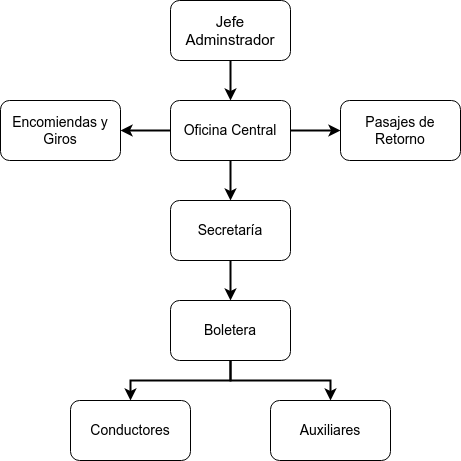
\includegraphics[width=0.55\textwidth]{img/Organigrama.png} % Inserta una imagen
	
	\begin{flushleft}
		\hspace{1.20cm} \textbf{Nota.} Organigrama obtenido en entrevista con el administrador. % Nota al pie para esta figura
	\end{flushleft}
	\vspace{-16pt}
	\label{fig:figura2_1} % Etiqueta para referencia cruzada
\end{figure}

En la Figura 1, se observa la estructura organizativa del negocio, destacando los diferentes cargos que desempeñan los empleados, que van desde el administrador hasta los auxiliares de apoyo. Dentro del negocio, se encuentran los boleteros y conductores, quienes son responsables de la atención directa a los pasajeros y la operación de los vehículos. Paralelamente, en la oficina central se gestionan las encomiendas, que son recibidas, clasificadas y preparadas para su envío. Cada uno de estos roles desempeña una función esencial para el funcionamiento eficiente y efectivo de la empresa, asegurando que tanto el transporte de pasajeros como la gestión de encomiendas se realicen con éxito y dentro de los estándares de calidad establecidos.

\subsection*{Misión de la empresa}

Proporcionar servicios de transporte y logística de alta calidad, enfocándose en la venta de pasajes y el envío de encomiendas, con el objetivo de satisfacer plenamente las necesidades de nuestros clientes. Nos comprometemos a ofrecer un servicio eficiente, seguro y confiable, contribuyendo al bienestar y comodidad de nuestros usuarios.

\subsection*{Visión de la empresa}

Ser la empresa líder en el sector del transporte y la logística en Bolivia, reconocida por nuestra innovación, eficiencia operativa y excelencia en el servicio al cliente. Aspiramos a expandir nuestra presencia y mejorar continuamente nuestros servicios para mantenernos a la vanguardia de la industria.

\subsection*{Objetivo general de la empresa}
El objetivo general de Cali Internacional es consolidar y expandir nuestra posición en el mercado del transporte y la logística, mejorando continuamente la calidad de nuestros servicios y adoptando tecnologías avanzadas para optimizar nuestras operaciones y satisfacer las necesidades cambiantes de nuestros clientes.

\subsection*{Objetivos específicos de la empresa}

\begin{itemize}[label=$\bullet$, left=0cm, labelsep = 1.05cm, topsep = 0pt, parsep = 0pt]
	
	\item Mejorar la experiencia del cliente mediante la oferta de servicios más rápidos, seguros y fiables.
	
	\item Capacitar continuamente a nuestro personal para asegurar que estén equipados con las habilidades necesarias para manejar las nuevas tecnologías y brindar un servicio de alta calidad.
	
	\item Implementar prácticas sostenibles en nuestras operaciones, minimizando el impacto ambiental y promoviendo la responsabilidad social corporativa.
	
\end{itemize}

\subsection{Antecedentes de proyectos similares}

Para la presente investigación se han considerado los siguientes antecedentes:

\textcite{hurtado2019aplicacion}. ``Aplicación web administrativa para reserva de servicios de transporte y envío de encomiendas para la empresa Romero y Asociados (AMBASEUR) de la ciudad de Ambato''. En este proyecto, se implementó una aplicación web para automatizar los procesos manuales de una empresa, mejorando la gestión de reservas de transporte y envíos de encomiendas. La plataforma permite publicitar las actividades de la empresa y recopilar información precisa sobre los clientes. Desarrollada utilizando la metodología XP, la aplicación facilita la adaptación rápida a cambios y la incorporación de funciones adicionales, como un chat en línea, optimizando así la eficiencia y aumentando la base de clientes.

\textcite{mora2022sistema}. ``Sistema gestión de servicio de viajes para la empresa Nuestra Señora de la Asunción C.I.S.A.'', esta investigación se centra en automatizar los procesos manuales de la empresa Nuestra Señora de la Asunción CISA mediante un sistema informático. En la primera etapa, se diagnosticaron los módulos de viajes, tráfico y ventas, entrevistando a responsables clave y recopilando los requerimientos necesarios. En la segunda etapa, se desarrolló un sistema informático web responsive que procesa automáticamente la información de estos módulos, integrando análisis, diseño y programación orientada a objetos, culminando en un sistema integrado con soporte audiovisual.

\textcite{arevalo2021desarrollo}. ``Desarrollo de una aplicación web para
agilizar los procesos de la compra y venta de boletos de buses interprovinciales en el terminal de Milagro.'', este proyecto desarrolló un sistema web para la compra y venta de boletos en el terminal terrestre del Cantón Milagro, con el objetivo de agilizar el proceso de boletería sin necesidad de contacto físico en ventanilla. Tras entrevistar a los socios del terminal para identificar los requisitos funcionales y no funcionales, se eligió la metodología ágil SCRUM para la organización y monitoreo constante del proyecto. El sistema se implementó utilizando Python, con Pycharm como IDE, Bootstrap 4 y Adminlte3 como plantillas, y PostgreSQL como base de datos. El resultado fue un sistema que satisface las necesidades del cliente, mejorando significativamente la experiencia de compra de boletos..

\textcite{sosa2019sistema}. ``Sistema informático web para la gestión de pasajes de la empresa de transporte Turismo Transol Barranca S.A.C.'', en la tesis se propone como objetivo principal desarrollar un sistema informático web para la gestión de pasajes en la empresa de transportes Turismo Transol Barranca S.A.C., abarcando tanto la venta como la reserva de boletos. Este sistema busca optimizar el tiempo de procesamiento mediante el uso de tecnología web. La investigación se llevó a cabo con un enfoque descriptivo, un diseño no experimental y un corte transversal, utilizando una población de 42 personas y una muestra de 6 usuarios. Se aplicó la metodología Proceso Unificado de Rational (RUP), empleando el Lenguaje de Modelamiento Unificado (UML) para la construcción de diagramas de casos de uso, facilitando el análisis del software. El sistema fue desarrollado en Java, con MySQL como gestor de datos y MySQL Workbench 6.3 CE para el modelado de la base de datos, entre otras herramientas que ayudaron a cumplir los requisitos de diseño. Los resultados permitieron agilizar los procesos de venta y reserva de pasajes, mejorando el manejo de la información y extendiendo el alcance a los clientes, lo que fortaleció el posicionamiento competitivo de la empresa a nivel regional.

\textcite{vivas2019propuesta}. ``Propuesta de implementación del sistema web de venta de boletos de viaje y gestión de encomiendas para la empresa Transportes Montero S.A.C. Piura; 2018.'', en esta investigación que fue desarrollada por la Escuela Profesional de Ingeniería de Sistemas de la Universidad Católica Los Ángeles de Chimbote, se centró en la mejora de procesos en organizaciones peruanas mediante la implementación de un sistema web para la venta de boletos y gestión de encomiendas en la empresa TRANSPORTES MONTERO S.A.C. en 2018. La investigación, de tipo cuantitativo y descriptivo con diseño no experimental y corte transversal, incluyó una muestra de 14 trabajadores. Los resultados mostraron que el 63 por ciento de los empleados consideraba que la empresa brindaba calidad en procesos y servicios, el 84 por ciento creía que los sistemas web agilizan los procesos, y el 81 por ciento opinaba que dichos sistemas eran eficientes, confirmando así la hipótesis planteada.

\section{OBJETO DE ESTUDIO}

Software de logística y gestión de buses para transporte de pasajeros y envío de encomiendas, el cual va automatizar y mejorar la eficiencia en la reserva y compra de pasajes, así como en la recepción, procesamiento y envío de encomiendas.

\section{PLANTEAMIENTO DEL PROBLEMA}

La empresa de transporte Cali Internacional, se encuentra ante diversos retos importantes en cuanto a administrar sus procesos tanto de venta de pasajes como de envío de paquetería, estas operaciones son llevadas a cabo de forma manual, lo que genera ineficiencias en el funcionamiento, largos tiempos de espera para los clientes y una alta posibilidad de comoter errores. Además de afectar negativamente la experiencia del cliente, estos problemas también restringen las posibilidades de crecimiento y competencia efectiva en un mercado cada vez más digital, la implementación de soluciones tecnológicas integrales se ha convertido en una estrategia clave para optimizar procesos.  

Algunos de los problemas mas frecuentes son:

\begin{itemize}[label=$\bullet$, left=1.25cm, labelsep = 0.75cm, topsep = 0pt, parsep = 0pt]
	\item Largos tiempos de espera en la compra de pasajes y envío de encomiendas debido a la falta de automatización.
	\item Errores en la gestión de reservas y envíos, lo que puede resultar en pérdidas financieras y descontento entre los clientes.
	\item Falta de visibilidad y control sobre la demanda de servicios, lo que limita la capacidad de la empresa para ajustar su oferta y optimizar recursos.
	\item Dificultad para generar reportes y análisis que ayuden en la toma de decisiones estratégicas para la empresa.    
\end{itemize}

Por lo tanto, se plantea la siguiente interrogante:

?`Cómo mejorar la venta de pasajes y la gestión de envío de encomiendas en la empresa Cali Internacional?

\section{JUSTIFICACIÓN}

La implementación de un software de logística y gestión de buses para transporte de pasajeros y envío de encomiendas representa una respuesta estratégica ante la creciente demanda de soluciones tecnológicas en el sector de transporte y logística. La automatización de estos procesos no solo optimiza las operaciones internas, sino que también reduce significativamente los errores humanos y mejora la eficiencia. En vista de ello la mayoría de organizaciones se ha visto obligada a desarrollar un sistema web de calidad que brinde un mejor servicio a la comunidad, mejorando su imagen corporativa, demostrando que están al día con las nuevas tecnologías \parencite{nunez2005diseno}.

Además, este proyecto aborda la necesidad de ofrecer un servicio más accesible y conveniente para los clientes. En un entorno donde la digitalización se ha vuelto imprescindible, la adopción de un sistema informático para estos servicios es una ventaja competitiva que no se puede ignorar.

La digitalización de estos procesos en una plataforma única no solo agilizará las operaciones al automatizar tareas repetitivas y reducir la necesidad de intervención manual, sino que también mejorará significativamente la precisión y la transparencia de la información. Esta mejora permitirá a la empresa ofrecer un servicio más coherente y eficiente, ya que todos los datos estarán centralizados y accesibles en tiempo real, lo que facilitará una gestión más efectiva de los recursos. Además, la integración de estos procesos en una sola plataforma reducirá costos operativos al eliminar redundancias y optimizar el uso de la infraestructura tecnológica. En última instancia, esto resultará en una mejor experiencia para el cliente, aumentando su satisfacción al recibir un servicio más rápido y confiable, y posicionando a la empresa como líder en innovación y eficiencia dentro de su sector.

Este proyecto se adapta a la necesidad de mantenerse al día con las tendencias tecnológicas actuales. Las empresas están siendo revolucionadas por la transformación digital, y aquellas que no se adapten corren el riesgo de quedarse atrás. Cuando la empresa implementa un software especializado, no solo se adapta a estas tendencias, sino que también está preparada para hacer frente a los desafíos futuros como la necesidad de incorporar nuevas tecnologías y responder a las demandas del mercado en constante cambio.

\section{OBJETIVOS}

\subsection{Objetivo general}

Desarrollar un software de logística y gestión de buses para transporte de pasajeros y envío de encomiendas para la empresa Cali Internacional de la ciudad de La Paz.

\subsection{Objetivos específicos}

\begin{itemize}[label=$\bullet$, left=0cm, labelsep = 1.05cm, topsep = 0pt, parsep = 0pt]

	\item Analizar los procesos actuales de venta de pasajes y envío de encomiendas en la empresa Cali Internacional para identificar las áreas de mejora y las necesidades tecnológicas específicas.
	\item Diseñar una interfaz de usuario intuitiva y accesible que permita a los empleados y clientes interactuar con el sistema de manera sencilla, facilitando la usabilidad del software.
    \item Elaborar el diseño de la base de datos a partir del análisis de los requerimientos del sistema, para llevar a la Tercera Forma Normal (3FN) y almacenar los datos.
    \item Diseñar el back-end para gestionar la venta de pasajes y el envío de encomiendas, asegurando la integración eficiente con la base de datos y la correcta ejecución de las operaciones solicitadas por los usuarios a través de la plataforma digital.    
	\item Generar reportes y análisis de datos que facilite la toma de decisiones informadas por parte de la administración de la empresa.
    
\end{itemize}

\section{MATRIZ DEL MARCO LÓGICO}

\begin{spacing}{1.1}
%	\centering
	\footnotesize
	% Eliminar espacio antes y después de longtable
	% \setlength{\LTpre}{0pt}
	\setlength{\LTpost}{0pt}
	
	\begin{longtable}{| m{5.3cm} | m{2.9cm} | m{3.4cm} | m{3.4cm} | } % solo con \usepackage{array}		
		\hline
		\textbf{Resumen narrativo} & \textbf{Indicadores objetivamente verificables}  & \textbf{Medios de verificación} & \textbf{Supuestos} \\ 
		\hline  
		\textbf{Fin:}\newline Software para la venta de pasajes y envio de encomiendas para la empresa Cali Internacional. & & & Implementar el software de venta de pasajes \\
		\hline 
		
		\textbf{Propósito:}\newline Desarrollar e implementar un software para la venta de pasajes y la gestión de encomiendas para reducir los tiempos de ventas, para una buena toma de decisiones dentro la empresa Cali Internacional. & \textbf{Cantidad}\newline 5 Módulos\newline \textbf{Calidad}\newline ISO/IEC 9126 \newline \textbf{Tiempo} \newline Hasta Octubre 2024 & Defensa del proyecto de grado & Conectividad continua de internet para evitar pérdida de información \\
		\hline
		
		\textbf{Productos:}\newline		
		1. Analizar los procesos actuales de venta de pasajes y envío de encomiendas en la empresa Cali Internacional para identificar las áreas de mejora y las necesidades tecnológicas específicas. &  Se realizarán 4 entrevistas con el administrador para analizar los requerimientos de la empresa, sera en 2 semanas. & Conformidad de todos los requerimientos por parte del administrador & Requerimientos factibles
		para la implementación del software \\
		\hline
		
		2. Diseñar una interfaz de usuario intuitiva y accesible que permita a los empleados y clientes interactuar con el sistema de manera sencilla, facilitando la usabilidad del software. &  Se realizará 5 interfaces, con el respaldo de las reuniones con el personal de la empresa, hasta la
		segunda semana de septiembre. & Correcto funcionamiento de las interfaces con capturas de pantalla. & Datos adaptables para los formularios en la parte de la interfaz. \\
		\hline
		
		3. Elaborar el diseño de la base de datos a partir del análisis de los requerimientos del sistema, para llevar a la Tercera Forma Normal (3FN) y almacenar los datos. &  Se realizará 1 Base de Datos, en base a la 1a, 2a y 3a forma normal, hasta la tercera semana de agosto. & Correcto funcionamiento con datos reales dentro del gestor de base de datos. & Datos y registros reales de la empresa. \\
		\hline
		
		4. Diseñar el back-end para gestionar la venta de pasajes y el envío de encomiendas, asegurando la integración eficiente con la base de datos y la correcta ejecución de las operaciones solicitadas por los usuarios a través de la plataforma digital. & Se registrarán 3 roles con sus respectivos permisos, contara una encriptación de contraseña, hasta la
		última semana de septiembre. & Pruebas de autentificación
		por parte del administrador, encargado de ventas, producción y almacenes. & Administrador, encargado de ventas y conductores, todos con documentación en orden. \\
		\hline
		
		5. Generar reportes y análisis de datos que facilite la toma de decisiones informadas por parte de la administración de la empresa. &  Se realizará 5 reportes con el respaldo de las reuniones con el administrador y usuarios
		correspondientes para su verificación, hasta la última semana de
		octubre. & Generar reportes con datos reales y conformidad del Gerente. & Información real de los registros de ventas envío de encomiendas.\\
		\hline
		
		\textbf{Actividades:} & & & \\		
		1.1 Reuniones con el administrador.	& Se estima que las reuniones durarán 40 minutos en promedio en 1 semana. & Aceptación de reunión. & Disponibilidad de tiempo del administrador.\\
		\hline
		1.2 Identificar los requerimientos funcionales. & Se estima 2 días para la identificación. & Notas guardadas de la reunión. & Requerimientos factibles.\\
		\hline				
		2.1 Diseñar el modelo vista-template del módulo de registro e inicio de sesión de usuarios, que tendrá formularios, interfaces y rutas. & Se culminará en aproximadamente 2 semanas. & Conformidad de los
		usuarios al momento del funcionamiento de la interfaz. & Framework en
		funcionamiento.\\
		\hline
		2.2 Diseñar el modelo vista-template del módulo de administración de usuarios, que tendrá formularios, interfaces y rutas. & Se realizará
		aproximadamente en 1 semana. & Conformidad del administrador y los
		usuarios al momento del funcionamiento de la interfaz. & Framework en
		funcionamiento. \\
		\hline
		2.3 Diseñar el modelo vista-template del módulo de autenticación de usuarios, que tendrá formularios, interfaces, ruta y token de seguridad. & Se llevará a cabo en aproximadamente 2 semanas. & Conformidad del administrador y los usuarios al momento del funcionamiento de la interfaz. & Framework en funcionamiento. \\
		\hline
		2.4 Diseñar el modelo vista-template del módulo de administración de
		ventas, que tendrá formularios, interfaces y rutas. & Se concretará en aproximadamente 3 semanas. & Conformidad del  administrador y los usuarios al momento del funcionamiento de la interfaz. & Framework en funcionamiento.\\
		\hline
		2.5 Prueba de interfaces con la presencia y participación del personal. & Se llevará a efecto en aproximadamente 2 días. & Aceptación de los módulos por parte del personal. & Interfaces finalizadas en un correcto funcionamiento. \\
		\hline
		
		3.1 Identificar la información necesaria de la reunión. & Se estima 1 día para identificación. & Notas con la información más relevante. & Información clara y concreta.\\
		\hline
		3.2 Diseñar el modelo entidad relación y el modelo relacional. & Se realizará en 2 días. & Modelos claros y sin errores. & Conocimiento de diseño de base de datos.\\
		\hline
		3.3 Diseñar la base de datos dentro del gestor. & Tomará 1 día el registro en el gestor. & Base de datos funcional con capturas de pantalla. & Gestor en correcto funcionamiento.\\
		\hline
		3.4 Normalizar la base de datos. & Se culminará en 1 día la normalización. & Base de datos normalizada y funcional con capturas de pantalla. & Conocimiento en normalización de base de datos.\\
		\hline
		3.5 Pruebas de funcionamiento con datos reales. & Se efectuará las pruebas en 1 día. & Capturas de pantalla del funcionamiento de la base de datos. & Cargado de datos reales a la base de datos.\\
		\hline
		
		4.1 Implementar la seguridad de la información de la base de datos. & Se llevará adelante en aproximadamente 1 semana. & Pruebas de seguridad mediante la gestión de usuarios del gestor de la base de datos. & Base de datos funcional con datos reales.\\
		\hline
		4.2 Implementar los roles con sus respectivas asignaciones. & Se llevará a término en aproximadamente 3 días. & Reuniones con el personal para asignar usuarios y contraseñas. & Personal identificado correctamente.\\
		\hline
		4.3 Pruebas de rendimiento de los roles con el personal. & Se concretará en 1 día. & Aceptación por parte del personal con el funcionamiento correcto de los roles asignados. & Disponibilidad de tiempo del personal.\\
		\hline
		
		5.1 Diseñar el modelo vista-controlador del módulo reportes, que tendrá formularios, interfaces, rutas y gráficos estadísticos. & Se llevará a efectividad en aproximadamente 4 semanas. & Conformidad del administrador al momento del funcionamiento de la interfaz. & Framework en funcionamiento.\\
		\hline
		5.2 Prueba de interfaces con la presencia y participación del Gerente. & Se efectuará en aproximadamente 2 días. & Aceptación de los módulos por parte del administrador. & Interfaces finalizadas en un correcto funcionamiento. \\
		\hline
		5.3 Subir el proyecto a un servidor y realizar las pruebas de funcionamiento. & Se llevará a cabo en aproximadamente 1 semana. & Software en funcionamiento en la nube. & Proyecto en correcto funcionamiento y finalizado. \\
		\hline		
	\end{longtable} 
\end{spacing}
\normalsize
\section{ALCANCES Y LÍMITES}
\subsection{Alcances}

El desarrollo de la presente investigación se encuentra dentro de los siguientes alcances:

\begin{itemize}[label=$\bullet$, left=0cm, labelsep = 1.05cm, topsep = 0pt, parsep = 0pt]

	\item El proyecto abarcará la creación de una plataforma digital que permita a los usuarios realizar la compra de pasajes y la gestión de envíos de encomiendas de manera eficiente y segura.

	\item Se desarrollará un sistema de gestión de usuarios que permitirá a los empleados: iniciar sesión y gestionar las ventas de pasajes y envíos de encomiendas, mientras que los administradores podrán supervisar y manejar las operaciones.

	\item Se implementarán módulos que automatizarán tareas repetitivas como la generación de recibos, el seguimiento de envíos y la asignación de asientos en los transportes.

	\item El sistema incluirá un módulo de reportes que permitirá a los administradores generar informes detallados sobre las ventas, la ocupación de los transportes, y la gestión de encomiendas.

	\item La plataforma será accesible desde diferentes tipos de dispositivos, incluyendo computadoras, tabletas, y smartphones, garantizando una experiencia de usuario consistente y accesible.

\end{itemize}

\subsection{Límites}

Los límites de la investigación son los siguientes:

\begin{itemize}[label=$\bullet$, left=0cm, labelsep = 1.05cm, topsep = 0pt, parsep = 0pt]

	\item El sistema estará diseñado inicialmente para cubrir las operaciones de la Empresa Cali Internacional en su sede de la Terminal de Buses en La Paz.
	
	\item La integración se centrará en los sistemas internos existentes de la empresa. %dejando de lado conexiones con plataformas o sistemas externos.
	
	\item El software será compatible con las plataformas y dispositivos especificados. %sin incluir soporte para otros sistemas no contemplados inicialmente.
	
	\item El soporte se limitará a las funcionalidades implementadas, las actualizaciones o desarrollos adicionales quedarán para fases futuras.

	% \item El proyecto no incluirá funcionalidades avanzadas de comunicación, como chat en tiempo real entre usuarios y administradores, limitando la interacción a métodos tradicionales.
	
\end{itemize}

%La venta de pasajes y la gestión de encomiendas tradicionalmente han sido procesos separados y manuales, lo que a menudo resulta en ineficiencias y errores debido a la falta de integración y la posibilidad de duplicación de esfuerzos. Estas ineficiencias pueden manifestarse en forma de retrasos en el procesamiento, errores humanos en la documentación y dificultades en el seguimiento de las transacciones. 

\section{METODOLOGÍA}

Para el desarrollo del proyecto se toma el modelo en cascada, que segun \cite{pressman1998ingenieria}, el modelo de cascada también conocido como modelo lineal secuencial, se basa en un enfoque sistemático y secuencial para el desarrollo del software que comienza en un nivel de sistemas y progreso con el análisis, diseño, implementación o codificación, pruebas y mantenimiento.

“Modelo de la cascada, se aplica por lo general cuando los requerimientos se
comprenden bien desde la comunicación hasta el despliegue; y sugiere un enfoque sistemático y secuencial para el desarrollo de software. Es un enfoque metodológico que ordena de manera rigurosa las etapas del ciclo de vida del software, de manera que cada inicio de etapa debe esperar la finalización de la inmediata anterior.” \parencite{pressman2010ingenieria}

Por su parte \cite{sommerville2011introduccion} destaca al modelo en cascada como “un ejemplo de un proceso dirigido por un plan; en principio, usted debe planear y programar todas las actividades del proceso, antes de comenzar a trabajar con ellas”, puntualizando de la siguiente manera las etapas de este modelo:

\begin{enumerate}[nosep, left=0cm, labelsep = 1cm]
	
	\item \textbf{Análisis y definición de requerimientos.} Los servicios, las restricciones y las metas del sistema se establecen mediante consulta a los usuarios del sistema. Luego, se definen con detalle y sirven como una especificación del sistema.	
	\item \textbf{Diseño del sistema y del software.} El proceso de diseño de sistemas asigna los requerimientos, para sistemas de hardware o de software, al establecer una arquitectura de sistema global. El diseño del software implica identificar y describir las abstracciones fundamentales del sistema de software y sus relaciones.
	\item \textbf{Implementación y prueba de unidad.} Durante esta etapa, el diseño de software se rea liza como un conjunto de programas o unidades del programa. La prueba de unidad consiste en verificar que cada unidad cumpla con su especificación.
	\item \textbf{Integración y prueba de sistema.} Las unidades del programa o los programas individuales se integran y prueban como un sistema completo para asegurarse de que se cumplan los requerimientos de software. Después de probarlo, se libera el sistema de software al cliente.
	\item \textbf{Operación y mantenimiento.} Por lo general (aunque no necesariamente), ésta es la fase más larga del ciclo de vida, donde el sistema se instala y se pone en práctica. El mantenimiento incluye corregir los errores que no se detectaron en etapas anteriores del ciclo de vida, mejorar la implementación de las unidades del sistema e incrementar los servicios del sistema conforme se descubren nuevos requerimientos.
\end{enumerate}

\section{IMPORTANCIA DEL ESTUDIO}

La importancia del estudio del proyecto radica en la necesidad de modernizar los procesos operativos de empresas de transporte y logística, especialmente en un entorno donde la eficiencia y la rapidez son factores clave para la competitividad. En la actualidad, muchas empresas en este sector aún dependen de sistemas manuales o desactualizados que ralentizan las operaciones, sino que también incrementan el riesgo de errores humanos, afectando directamente la calidad del servicio ofrecido al cliente. Este proyecto, por lo tanto, no solo aborda una necesidad tecnológica, sino que también busca mejorar la experiencia del cliente al ofrecerle un servicio más ágil y fiable.

Desde una perspectiva social, este estudio tiene una importancia significativa al contribuir al avance tecnológico en un sector que afecta directamente a un gran número de personas. Al mejorar la eficiencia y la precisión en la venta de pasajes y el envío de encomiendas, se generan beneficios directos no solo para la empresa, sino también para los usuarios finales, quienes experimentarán un servicio más confiable y accesible. Esto, a su vez, puede fomentar una mayor confianza en los servicios digitales en general, impulsando el uso de la tecnología en otras áreas de la vida diaria.

Finalmente, la importancia de este estudio también reside en su capacidad para servir como modelo para futuras implementaciones tecnológicas en empresas similares. La metodología empleada, así como los desafíos superados durante el desarrollo del software, pueden ofrecer valiosas lecciones para otros proyectos dentro del sector, promoviendo un enfoque más sistemático y eficiente en la adopción de tecnologías de la información en la industria del transporte y la logística.

\section{PUNTOS DE PROYECTO DE GRADO}

\noindent \textbf{CAPÍTULO I}

\noindent INTRODUCCIÓN

\begin{enumerate}[nosep, label=1.\arabic*., left = 0pt .. \parindent]
    \item ANTECEDENTES
    \begin{enumerate}[nosep, label=1.\arabic{enumi}.\arabic*., left = 0pt .. \parindent]
    	\item Antecedentes institucionales
    	\item Antecedentes de proyectos similares
    \end{enumerate}
    \item OBJETO DE ESTUDIO
    \item PLANTEAMIENTO DEL PROBLEMA
    \item JUSTIFICACIÓN
    \item OBJETIVOS
    \begin{enumerate}[nosep, label=1.\arabic{enumi}.\arabic*., left = 0pt .. \parindent]
    	\item Objetivo general
        \item Objetivos específicos
    \end{enumerate}
    \item ALCANCES Y LÍMITES
    \begin{enumerate}[nosep, label=1.\arabic{enumi}.\arabic*., left = 0pt .. \parindent]
    		\item Alcances
        \item Límites
    \end{enumerate}
    \item IMPORTANCIA DEL ESTUDIO
\end{enumerate}

\noindent CAPÍTULO II

\noindent MARCO TEÓRICO

\begin{enumerate}[nosep, label=2.\arabic*., left = 0pt .. \parindent]
    \item INGENIERÍA DE SOFTWARE
    \begin{enumerate}[nosep, label=2.\arabic{enumi}.\arabic*., left = 0pt .. \parindent]
    	\item Concepto
        \item Sobre la ingeniería de software
        \item Ingeniería de software en la actualidad
    \end{enumerate}
    \item MODELO DE CASCADA
    \begin{enumerate}[nosep, label=2.\arabic{enumi}.\arabic*., left = 0pt .. \parindent]
    	\item Requerimientos del software
        \item Diseño del programa
        \item Codificación
        \item Construcción de pruebas
        \item Implantación
    \end{enumerate}
    \item INGENIERÍA DE REQUERIMIENTOS
    \item MODELO ENTIDAD - RELACIÓN
    \item BASE DE DATOS
    \item DISEÑO DE LA INTERFAZ
    \begin{enumerate}[nosep, label=2.\arabic{enumi}.\arabic*., left = 0pt .. \parindent]
    	\item Frontend y backend
        \item Cabecera o header
        \item Cuerpo o body
        \item Pie de página o footer
    \end{enumerate}
    \item PROGRAMACIÓN
    \item HERRAMIENTAS DE DESARROLLO
    \item PRUEBAS
    \item IMPLANTACIÓN DEL SOFTWARE
    \item SEGURIDAD
    \begin{enumerate}[nosep, label=2.\arabic{enumi}.\arabic*., left = 0pt .. \parindent]
    	\item Encriptación
        \item Autenticación
	\end{enumerate}
	\item MODELO DE CALIDAD BOEHM
	\begin{enumerate}[nosep, label=2.\arabic{enumi}.\arabic*., left = 0pt .. \parindent]
		\item Usabilidad
		\item Portabilidad
	\end{enumerate}
    
\end{enumerate}

\noindent CAPÍTULO III

\noindent MARCO APLICATIVO

\begin{enumerate}[nosep, label=3.\arabic*., left = 0pt .. \parindent]
    \item ANÁLISIS Y DEFINICIÓN DE REQUERIMIENTOS
    \item DISEÑO DEL SISTEMA Y DEL SOFTWARE
    \item IMPLEMENTACIÓN Y PRUEBA DE UNIDAD
    \item INTEGRACIÓN Y PRUEBA DEL SISTEMA
    \item OPERACIÓN Y MANTENIMIENTO
    \item SEGURIDAD DE SOFTWARE
    \item NORMAS DE CALIDAD
    \item RESULTADOS
\end{enumerate}

\noindent CAPÍTULO IV

\noindent CONCLUSIONES Y RECOMENDACIONES

\begin{enumerate}[nosep, label=4.\arabic*., left = 0pt .. \parindent]
    \item CONCLUSIONES
    \item RECOMENDACIONES
\end{enumerate}


\section{BIBLIOGRAFÍA}
\nocite{cuevas2023}
\printbibliography[heading=none]
\section{CRONOGRAMA}

\begin{spacing}{1}
%\begin{table}[h]
%    \centering
    \footnotesize
\begin{longtable}{|p{4cm}|c|c|c|c|c|c|c|c|c|c|c|c|c|c|c|c|c|c|c|c|}\hline
\multirow{3}{*}{\textbf{Actividad}} & \multicolumn{20}{ |c| }{\textbf{DESDE JULIO HASTA NOVIEMBRE DEL 2024}} \\ 
\cline{2-21}
 & \multicolumn{4}{ |c| }{\textbf{JULIO}} & \multicolumn{4}{ |c| }{\textbf{AGOSTO}} & \multicolumn{4}{ |c| }{\textbf{SEPTIEMBRE}} & \multicolumn{4}{ |c| }{\textbf{OCTUBRE}} & \multicolumn{4}{ |c| }{\textbf{NOVIEMBRE}} \\ 
\cline{2-21}
& 1 & 2 & 3 & 4 & 1 & 2 & 3 & 4 & 1 & 2 & 3 & 4 & 1 & 2 & 3 & 4 & 1 & 2 & 3 & 4 \\ 
\hline 
1.1 Reuniones con el administrador.	& & \cellcolor{lightcopper} & \cellcolor{lightcopper} & & & & & & & & & & & & & & & & & \\ 
\hline 
1.2 Identificar los requerimientos funcionales. & & & & \cellcolor{lightcopper} & & & & & & & & & & & & & & & & \\ 
\hline 
2.1 Diseñar el modelo vista-template del módulo de registro e inicio de sesión de usuarios, que tendrá formularios, interfaces y rutas. & & & & & \cellcolor{skyblue6} & & & & & & & & & & & & & & & \\ 
\hline 
2.2 Diseñar el modelo vista-template del módulo de administración de usuarios, que tendrá formularios, interfaces y rutas. & & & & & & \cellcolor{skyblue6} & & & & & & &  &  &  & & & & & \\ 
\hline 
2.3 Diseñar el modelo vista-template del módulo de autenticación de usuarios, que tendrá formularios, interfaces, ruta y token de seguridad. & & & & & & & \cellcolor{skyblue6} & & & & & & & & & & & & & \\ 
\hline
2.4 Diseñar el modelo vista-template del módulo de administración de ventas, que tendrá formularios, interfaces y rutas.	& & & & & & & & \cellcolor{skyblue6} & & & & & & & & & & & & \\ 
\hline 
2.5 Prueba de interfaces con la presencia y participación del personal. & & & & & & & & \cellcolor{skyblue6} & & & & & & & & & & & & \\ 
\hline 
3.1 Identificar la información necesaria de la reunión. & & & & & & & & & \cellcolor{saffron} & & & & & & & & & & & \\ 
\hline 
3.2 Diseñar el modelo entidad relación y el modelo relacional. & & & & & & & & & & \cellcolor{saffron} & & & & & & & & & & \\ 
\hline 
3.3 Diseñar la base de datos dentro del gestor. & & & & & & & & & & & \cellcolor{saffron} & \cellcolor{saffron} & & & & & & & & \\ 
\hline 
3.4 Normalizar la base de datos. & & & & & & & & & & & & & \cellcolor{saffron} & & & & & & & \\ 
\hline 
3.5 Pruebas de funcionamiento con datos reales. & & & & & & & & & & & & & \cellcolor{saffron} & & & & & & & \\ 
\hline 
4.1 Implementar la seguridad de la información de la base de datos. & & & & & & & & & & & & & \cellcolor{darkseagreen} & \cellcolor{darkseagreen} & & & & & & \\ 
\hline 
4.2 Implementar los roles con sus respectivas asignaciones. & & & & & & & & & & & & & & & \cellcolor{darkseagreen} & & & & & \\ 
\hline 
4.3 Pruebas de rendimiento de los roles con el personal. & & & & & & & & & & & & & & & & \cellcolor{darkseagreen} & & & & \\ 
\hline 
5.1 Diseñar el modelo vista-template del módulo reportes, que tendrá formularios, interfaces, rutas y gráficos estadísticos. & & & & & & & & & & & & & & & & & \cellcolor{pastelred} & & & \\ 
\hline 
5.2 Prueba de interfaces con la presencia y participación del Gerente. & & & & & & & & & & & & & & & & & & \cellcolor{pastelred} & & \\ 
\hline 
5.3 Subir el proyecto a un servidor y realizar las pruebas de funcionamiento. & & & & & & & & & & & & & & & & & & & \cellcolor{pastelred} & \cellcolor{pastelred} \\ 
\hline 

\end{longtable} 
%\end{table}
\end{spacing}
\end{document}

